%%%%%%%%%%%%%%%%%%%%%%%%%%%%%%%%%%%%%%%%%%%%%%%%%%%%
%\graphicspath{chapters/figures/}
\chapter{Execution Unit}
\label{chap_exu}

%%%%%%%%%%%%%%%%%%%%%%%%%%%%%%%%%%%%%%%%%%%%%%%%%%%%%%%%%%%
\section{Overview}
We have designed an execution unit that is capable of dealing with almost all the instructions present in the instruction set that has been given. Exceptions are the floating point operations, which requires speicific hardware that we decided not to include. It is worth mentioning that normally the \textit{MUL} operations are executed by dividing them in subsequently pipelined stages. Here, differently, in order to keep the 5 stages in the pipeline and not to alter the normal execution flow, this doe not take place. As a consequence, the maximum operating frequency will be heavily affected by the propagation time needed by the multiplier to finish its job.


In the \textit{Execution Unit} are therefore present the following components:
\begin{itemize}
	\item \textbf{shifter}, used in order to shift and rotate the value contained in an input register
	\item \textbf{adder}, necessary obviously to perform addition and subtraction between values, but also used in the logic comparison operations
	\item \textbf{logic}, unit to perform logic bitwise operations, such as \textit{OR, AND, XOR} and so on
	\item \textbf{comparator}, which purpose is to determine whether an input is greater, smaller or equal than another one
	\item \textbf{multiplier}, whose goal is to perform multiplications between inputs
	\item \text{PC adder}, a dedicated adder to increase by the value of the PC, useful in case of a \textit{JMP} operation
	\item \textbf{registers}, to update the inputs and store the results
	\item \textbf{muxes}, to select the results coming from the required unit and correctly update the outputs of the stage
	\item \textbf{inverter}, needed to perform the \textit{2'S complement} and perform the subtraction
\end{itemize}


For this stage, a bunch of bits of the \textsf{CW} are used. Here are reported:
\begin{itemize}
	\item \textit{ENEX}, a general enable for the components and especially for the registers
	\item \textit{MUX1\_SEL}, a selection signal for the mux that is able to select an immediate value or a register an input that as the first term for the other units
	\item \textit{MUX2\_SEL}, with a goal similar as the one above, but for the second input
	\item \textit{UN\_SEL}, 3 bits signal that selects the correct input, which is then sent to a register
	\item \textit{OP\_SEL}, 4 bits selection signal, used to indicate to each unit, with different encoding, the operation to be performed
	\item \textit{PC\_SEL}, selection signal to update the PC counter correctly, following a branch or jump.
\end{itemize}


\section{Adder}

For the adder architecture, we decided not to start from scratches. As long as our P4 adder, designed during the laboratories, has a general description, we resized it to our architecture on 32 bits. This means that we have included the components capable of producing the \textsf{PG} propagate and generate signals and the \textsc{G} ones used to produce only the generate and so the final carry. We consider that therefore the result, in terms of performance can satisfy us. At the input of the block, we have also a \textit{C\_IN} signal, which is used to create, in cooperation with the inverter, the \text{2'S complement} of the input used (either immediate or coming from a register), in order to produce as a final result the signed sum. There are few control signals used for this unit. In figure \ref{adder_fig} is presented the simple schematic of the adder block

\begin{figure}
	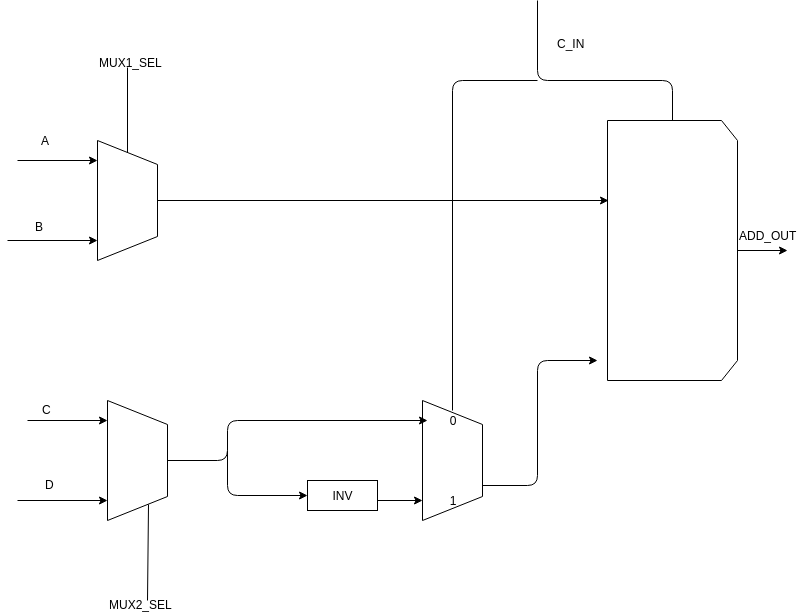
\includegraphics[width=\textwidth]{chapters/figures/adder}
	\caption{Adder with inverter and related selection signal}
	\label{adder_fig}
\end{figure}
